\section{Methods of Analysis}
Between the 21 individual studies conducted, there were not only a large variety of dependent and independent variables tracked, but a wide variety of methods employed to analyze the data collected over the course of the experiment.  We tracked every pairwise combination of independent and dependent variables that the experimenters recorded and whose effects were analyzed.  In regards to the user created hypotheses, we also recorded whether each method of analysis supported the initial hypothesis, rejected the initial hypothesis, or was inconclusive.  The employed methods are shown in Fig.\ref{fig:analysis}

\begin{figure}[!t]\centering
%\begin{wrapfigure}{o}{\textwidth}\centering
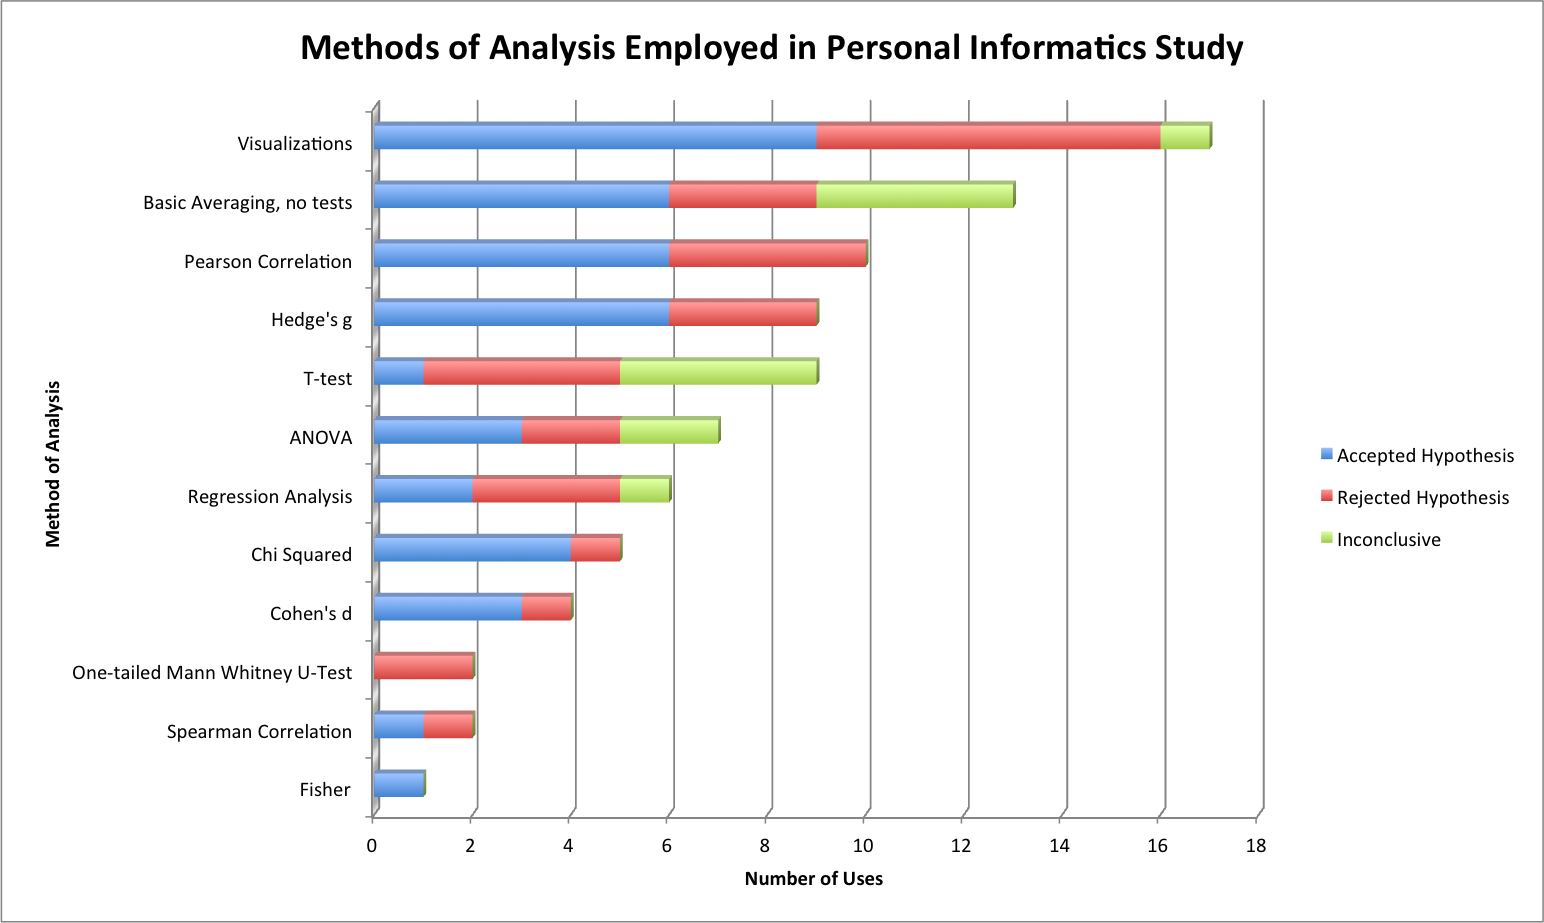
\includegraphics[width=1.0\columnwidth]{images/Methods_of_Analysis.png}
\caption{\footnotesize Employed methods of analysis \label{fig:analysis} 
}%\end{wrapfigure}
\end{figure}


Visualizations refers to the use of any graphs, plots, or other visual representations of the data collected and inferring relationships through mere observation.  This was the most popular method employed as many people used visualizations to accompany statistical tests they ran.  Of the visualizations, there was only one pairwise relationship whose effect, in regards to the user’s hypothesis, was deemed inconclusive.  Out of the 17 times these were used, 9 times the visualizations supported the hypotheses and 8 times they rejected the hypotheses.  While not all who used visualizations employed additional testing methods, given the test size of 1 and the relatively small time frame in which we conducted the experiments, it was considered acceptable to employ visualizations alone as a form of analysis. 

Basic averaging refers to the users who had to average some data points, usually per day or per session that they were tracking, and then comparing the average data.  This also required the use of no tests, however with dependent variables such as average heart rate throughout the duration of a work out, some users deemed this methods as the most appropriate way to gauge the existence or degree of an effect.  Of the 13 people who employed this method, 6 found their hypotheses to be supported, 3 found theirs to be rejected, and 4 found the data from averaging to be inconclusive.  In terms of variable such as heart rate, this may not have been the most effective way to see results.  Something such as average heart rate takes, usually, longer than 3-4 weeks to substantially change.  A better approach may have been to compare the high and low heart rates for each work, discarding the ascending and descending rate periods.  

Pearson’s correlation, or the correlation coefficient was used to measure the strength of the linear relationships between the independent and dependent variables.  Of the ten people to employ this method of analysis, there wasn’t a single person who found their results to be inconclusive.  This either supported the hypothesis, or rejected it.  This makes sense since there was no statistical test done on the actual correlation coefficient and so any correlation besides 0, which would be very unlikely to observe in scenarios such as these that are so dependent upon human behaviors, would render some sort of relationship. Out of these ten, 6 accepted and 4 rejected their hypotheses. 

As the fourth most common method of analysis employed, Hedge’s g also rendered no inconclusive results.  In terms of the effect size of independent variables on dependent variables, Hedge’s g had the same ratio that Pearson’s correlation did; 6 hypotheses were accepted and 4 were rejected.  As Hedge’s g reveals an effect and the size of that effect, it makes sense that hypotheses were either accepted or rejected, and that no one found their results to be inconclusive. 

While t-tests were the fifth most commonly used method of analysis, they were tied for the method that procured the most verdicts of inconclusive data.  Upon closer look, every user who employed a t-test used it to test the relationship between some dependent variable and either sleep quality or heart rate.  As both of these dependent variables are highly susceptible to a multitude of factors, all of which no one in the class recorded, it makes sense that those who used a t-test had the highest rate of finding their data inconclusive, as t-tests work best when there is large variance in the means of the data sets, a large sample size, and within the separate data sets, there is a low range, conditions not always applicable to heart rate and sleep quality, where in any given week there can be a wide range.  For individual experiments such as ours, a t-test may not have been the best method of analysis.

Seven pairwise relationships were tested using analysis of variance or ANOVA to gauge the effect of the dependent variable. This also had a proportionally high number of results rendered inconclusive to accept or reject the initial hypotheses. Of the seven, two were considered inconclusive, while two hypotheses were rejected and three were accepted. This makes sense as the basic ANOVA method generalizes a t-test to more than two sets.

As for the less common methods of analysis:
Regression analysis was used to test six hypotheses, two of which were accepted, three rejected and one accepted. 
Chi squared tests were used to test five hypotheses, four of which were accepted, and one rejected.
Cohen’s d was used to test the four hypotheses, three of which were accepted, one of which was rejected. 
A one-tailed Mann Whitney-U test was used for two hypotheses, both of which were rejected.
The Spearman Correlation was used for two hypotheses, one of which was accepted and one was rejected. 
Fisher’s exact test was used once, and it allowed the user to accept their hypothesis. 

From reading their reports and examining their respective findings, users seemed to have found drawing upon graphs and other visualizations very helpful in analyzing and then expressing their findings, in support of the statistical tests they ran.  In terms of small-scale studies such as ours, t-tests and ANOVA analysis seemed to procure a disproportionately large number of inconclusive verdicts, which we speculate is due to the small number of data points we collected, relative to larger, longer studies.

As far as detecting an actual effect and effect size, the testing methods that actually tested for size seemed to procure more definite results for our small scale testing, most prominently Hedge’s g. No doubt, as is later mentioned in our discussion, the varying backgrounds in statistics that were prevalent in our class affected the methods of analysis members employed.  The lesser used methods, such as the Spearman Correlation or Fisher’s exact test, are seldom taught, and not in depth, in introductory statistics classes, and thus those who had little background in or understanding of methods statistical analyses were at a disadvantage in terms of their methods of analysis. 
